\newpage
    \section{Auswertung}
    \subsection{Untergrund}
    Bevor eigentliche Messungen möglich sind, muss der Nulleffekt der Messungebung bestimmt werden. Diese einsteht zum Großteil aus natürlichen Strahlungen aus der Umgebung, wie zum Beispiel die Höhenstrahlung.
    Dieser wird in einem Messabstand von $t = \SI{300}{\second}$ zu:
    \begin{table}
	\centering
	\caption{Messdaten zum Nulleffekt}
	\label{tab:untergrundrate}
	\begin{tabular}{c c}
		\toprule
		$N_U$ & $\Delta N_U$ \\
		\midrule
		129 & 11.36 \\
		143 & 11.96 \\
		144 & 12 \\
		136 & 11.66 \\
		139 & 11.79 \\
		126 & 11.22 \\
		158 & 12.57 \\
		\bottomrule
	\end{tabular}
\end{table}
    Da die Untergrund Rate als Poissonverteilt, also die Messunsicherheit durch $\Delta N = \sqrt{N}$  gegeben ist, kann angenommen werden, dass diese gemittelt werden kann als:

    \begin{align*}
    N_\text{U} = 139.2857 \pm 11.8019.
    \end{align*}

    Diese Untergrundrate wird von jeder Messung abgezogen, um so die von der Quelle emitierten Teilchen lediglich zu betrachten.

    \subsection{Zerfallskurve und Halbwertszeit von Vanadium-52}
    \label{sec:vana}

    Nun wird die Zerfallskurve von Vanadium-52 betrachtet. Nach der Aktivierung wird der Teilchen Impuls $N$ alle $30 s$ gemessen. Damit folgen folgende Messergebnisse:
\begin{table}
	\centering
	\caption{Messdaten zum Zerfall von Vanadium-52.} 
	\label{tab:vana} 
	\begin{tabular}{c c c c}
	\toprule
	$t / \si{\second}$ & $N$ & $\Delta N$ &$N$ \\
	\midrule
		30   	&      189  	& 14.0 &      175.0 \\
		  60   	&      197  	& 14.0 &      183.0 \\
		  90   	&      150  	& 12.0 &      136.0 \\
		 120   	&      159  	& 13.0 &      145.0 \\
		 150   	&      155  	& 12.0 &      141.0 \\
		 180   	&      132  	& 11.0 &      118.0 \\
		 210   	&      117  	& 11.0 &      103.0 \\
		 240   	&      107  	& 10.0 &       93.0 \\
		 270   	&       94  	& 10.0 &       80.0 \\
		 300   	&      100  	& 10.0 &       86.0 \\
		 330   	&       79  	&  9.0 &       65.0 \\
		 360   	&       69  	&  8.0 &       55.0 \\
		 390   	&       81  	&  9.0 &       67.0 \\
		 420   	&       46  	&  7.0 &       32.0 \\
		 450   	&       49  	&  7.0 &       35.0 \\
		 480   	&       61  	&  8.0 &       47.0 \\
		 510   	&       56  	&  7.0 &       42.0 \\
		 540   	&       40  	&  6.0 &       26.0 \\
		 570   	&       45  	&  7.0 &       31.0 \\
		 600   	&       32  	&  6.0 &       18.0 \\
		 630   	&       27  	&  5.0 &       13.0 \\
		 660   	&       43  	&  7.0 &       29.0 \\
		 690   	&       35  	&  6.0 &       21.0 \\
		 720   	&       19  	&  4.0 &        5.0 \\
		 750   	&       28  	&  5.0 &       14.0 \\
		 780   	&       27  	&  5.0 &       13.0 \\
		 810   	&       36  	&  6.0 &       22.0 \\
		 840   	&       25  	&  5.0 &       11.0 \\
		 870   	&       29  	&  5.0 &       15.0 \\
		 900   	&       18  	&  4.0 &        4.0 \\
		 930   	&       17  	&  4.0 &        3.0 \\
		 960   	&       24  	&  5.0 &       10.0 \\
		 990   	&       21  	&  5.0 &        7.0 \\
		1020   	&       25  	&  5.0 &       11.0 \\
		1050   	&       21  	&  5.0 &        7.0 \\
		1080   	&       24  	&  5.0 &       10.0 \\
		1110   	&       25  	&  5.0 &       11.0 \\
		1140   	&       17  	&  4.0 &        3.0 \\
		1170   	&       20  	&  4.0 &        6.0 \\
		1200   	&       19  	&  4.0 &        5.0 \\
		1230   	&       20  	&  4.0 &        6.0 \\
		1260   	&       18  	&  4.0 &        4.0 \\
		1290   	&       16  	&  4.0 &        2.0 \\
		1320   	&       17  	&  4.0 &        3.0 \\
\bottomrule
	\end{tabular}
\end{table}
\noindent
Auch hier kann die Abweichung als Poisson Verteilung mit $\Delta N = \sqrt{N}$ angenommen werden. Zusätzlich wird die Untergrundsrate $14 \frac{\text{Zerfällen}}{\SI{30}{\second}}$ von jedem Messergeebnis abgezogen.

Für die im Zeitinterval $\Delta t$ gemessenen Zerfälle gilt
\begin{equation}
	\ln N_{\Delta t}(t) = \ln\left( N_0 \cdot \left(1 - e^{-\lambda \Delta t}\right) \right) - \lambda t.
	\label{eqn:logarithmisch}
\end{equation}
\noindent

Um einen Fit zu berechnen, kann eine lineare Ausgleichsrechnung in der Form
\begin{equation*}
	f(x) = m \cdot x + b
	\label{eqn:mx+b}
\end{equation*}
\noindent

genutzt werden, wenn die Daten logarithmisch betrachtet werden. So folgt aus dem Fit, dass

\begin{align*}
    m =& -0.00316 \pm 0.00016 \\
    b =& 5.18650 \pm  0.12753
\end{align*}

Mit Hilfe der Formel (\ref{eqn:logarithmisch}) ist der Zusammnehang zwischen $m$ und $\lambda$: $m = -\lambda$.
So folgt für 
\begin{align*}
	\lambda = (3.16 \pm 0.16) 10^{-3} \  \si{\second}^{-1}.
\end{align*}

Mit diesem Fit lassen sich die Daten in (\ref{fig:zerfallskurve3}) plotten:

\begin{figure}[H]
	\centering
	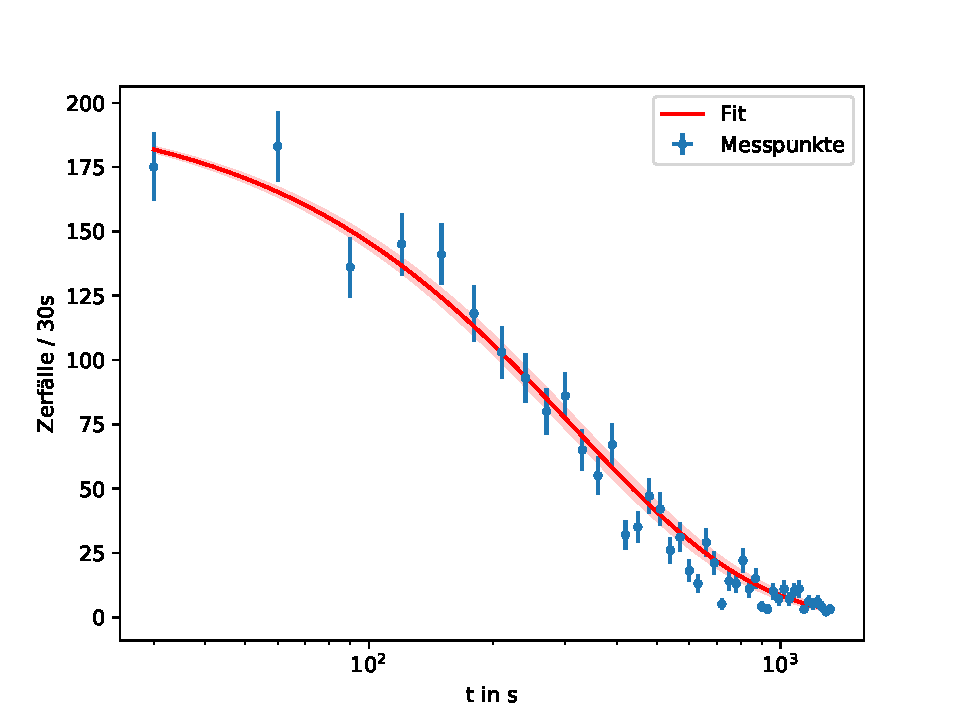
\includegraphics{Daten/Vanadium.pdf}
	\caption{Messdaten und Fit für die Zerfallskurve von Vanadium.}
	\label{fig:zerfallskurve3}
\end{figure}
\noindent

Mithilfe der Formel (\ref{eqn:T}) lässt sich die Halbwertszeit bestimmen zu:
\begin{align*}
	T = \SI{219\pm11}{\second}.
\end{align*}
\noindent

Da die Messdaten sich zum Ende der Messung kaum unterscheiden lassen, wird ein zweiter Fit durch die Daten gelegt, jedoch diesmal nur bis zum Zeitpunkt $t = \SI{300}{\second}$. Aus diesem
Fit folgt 
\begin{align*}
    m =& -0.00308 \pm 0.00029 \\
    b =& 5.30866 \pm  0.05512.
\end{align*}
\noindent
Daraus lässt sich die Halbwertszeit bestimmen zu:
\begin{align*}
	T = \SI{225\pm22}{\second}.
\end{align*}

\subsection{Zerfallskurve und Halbwertszeit von Rhodium-104}
Da Rhodium-104 in zwei unterschiedliche Kerne mit zwei unterscheidlichen Wahrscheinlichkeiten Zerfallen kann und diese in dem Moment der Messung nicht getrennt erfasst werden können,
muss in den foglenden Daten dieser Zerfall mit berücksichtigt werden.
\noindent
Aus der Messung folgen folgende Werte:
\begin{table}
	\centering
	\caption{Messdaten zum Zerfall von Rhodium-104.} 
	\label{tab:rhodium}
	\begin{tabular}{c c c c}
	\toprule
	$t / \si{\second}$ & $N$ & $\Delta N$ &$N$ Korrigiert \\
	\midrule
		15  	& 667  	& 26.0         	& 660.0 \\
		 30  	& 585  	& 24.0         	& 578.0 \\
		 45  	& 474  	& 22.0         	& 467.0 \\
		 60  	& 399  	& 20.0         	& 392.0 \\
		 75  	& 304  	& 17.0         	& 297.0 \\
		 90  	& 253  	& 16.0         	& 246.0 \\
		105  	& 213  	& 15.0         	& 206.0 \\
		120  	& 173  	& 13.0         	& 166.0 \\
		135  	& 152  	& 12.0         	& 145.0 \\
		150  	& 126  	& 11.0         	& 119.0 \\
		165  	& 111  	& 11.0         	& 104.0 \\
		180  	&  92  	& 10.0         	&  85.0 \\
		195  	&  79  	&  9.0         	&  72.0 \\
		210  	&  74  	&  9.0         	&  67.0 \\
		225  	&  60  	&  8.0         	&  53.0 \\
		240  	&  52  	&  7.0         	&  45.0 \\
		255  	&  56  	&  7.0         	&  49.0 \\
		270  	&  53  	&  7.0         	&  46.0 \\
		285  	&  41  	&  6.0         	&  34.0 \\
		300  	&  36  	&  6.0         	&  29.0 \\
		315  	&  37  	&  6.0         	&  30.0 \\
		330  	&  32  	&  6.0         	&  25.0 \\
		345  	&  36  	&  6.0         	&  29.0 \\
		360  	&  38  	&  6.0         	&  31.0 \\
		375  	&  34  	&  6.0         	&  27.0 \\
		390  	&  40  	&  6.0         	&  33.0 \\
		405  	&  21  	&  5.0         	&  14.0 \\
		420  	&  35  	&  6.0         	&  28.0 \\
		435  	&  33  	&  6.0         	&  26.0 \\
		450  	&  36  	&  6.0         	&  29.0 \\
		465  	&  20  	&  4.0         	&  13.0 \\
		480  	&  24  	&  5.0         	&  17.0 \\
		495  	&  30  	&  5.0         	&  23.0 \\
		510  	&  30  	&  5.0         	&  23.0 \\
		525  	&  26  	&  5.0         	&  19.0 \\
		540  	&  28  	&  5.0         	&  21.0 \\
		555  	&  23  	&  5.0         	&  16.0 \\
		570  	&  20  	&  4.0         	&  13.0 \\
		585  	&  28  	&  5.0         	&  21.0 \\
		600  	&  17  	&  4.0         	&  10.0 \\
		615  	&  26  	&  5.0         	&  19.0 \\
		630  	&  19  	&  4.0         	&  12.0 \\
		645  	&  13  	&  4.0         	&   6.0 \\
		660  	&  17  	&  4.0         	&  10.0 \\
		\bottomrule
	\end{tabular}
\end{table}
\noindent
Auch hier kann die Messunsicherheit als Poisson Verteilung mit $\Delta N = \sqrt{N}$ angenommen werden. Um die Untergrundsrate mit zu berücksichtigen wird diese im (\ref{sec:vana}) ebenfalls 
mitabgezogen.
\noindent
Da der schnelle Zerfall vom langsamen Zerfall überlagert wird, muss dieser als erstes betrachtet werden. Um die Überlagerung zu kompensieren werden zunächst die Messdaten ab 
$t = \SI{330}{\second}$ betrachtet.
Das vorgehen ist dem in Kaptiel (\ref{sec:vana}) gleich. 
\noindent
Zunächst werden die Daten Halblogarithmisch betrachtet und es wird mit Hilfe der Funktion (\ref{eqn:mx+b}) ein Fit durchgelegt. Aus diesem folgt:
\begin{align*}
    m =& -0.00323 \pm 0.00073 \\
    b =& 5.34146 \pm  0.34622.
\end{align*}

Aus dem Zusammnehang $m = -\lambda$ lässt sich die Halbwertszeit von Rhodium-104 bestimmen zu:
\begin{align*}
	T = 2.1\pm0.5 10^{2} \si{\second}.
\end{align*}

Mithilfe der Daten und der Ausgleichsgerade wird die folgende Grafik geplottet:
\begin{figure}[H]
	\centering
	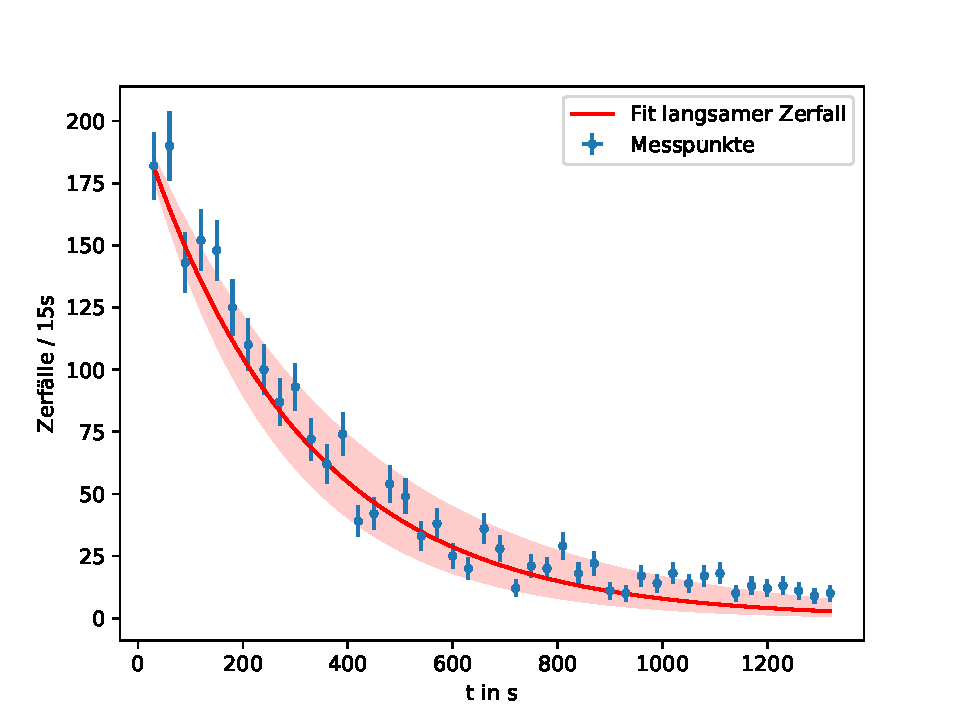
\includegraphics{Daten/Rhodium.pdf}
	\caption{Messdaten und Fit für die Zerfallskurve von Rhodium.}
	\label{fig:zerfallskurve}
\end{figure}
\noindent
\newpage
Nun kann die Zerfallsrate von dem schnellen Zerfall betrachtet werden. Dafür wird mit $T_\text{l}$ berechnet, wie viele Impulse pro Messintervall am Anfang durch den schnellen Zerfall ausgelöst wurden.
Dies kann Mithilfe des Zerfallgesetztes bestimmt werden zu:
\begin{equation}
	N_{\Delta t_\text{l}} (t) = N_{0_\text{l}} \left(1 - e^{-\lambda_\text{l}\Delta t}\right) 
	e^{-\lambda_\text{l}t }.
\end{equation}
\noindent

Wird $N_{\Delta t_\text{l}}$ von den Messdaten bis $\SI{150}{\second}$ abgezogen und lediglich diese auch betrachtet, kann die Impulsrate des schnellen Zerfalls durch:
\begin{equation*}
	\{ \ln(N_{\Delta t}(t_i) - N_{\Delta t_\text{l}} (t_i)) \}
\end{equation*}
berchnet und gefittet werden. Daraus folgt für die Funktion (\ref{eqn:mx+b})
\begin{align*}
    m =& -0.00285 \pm 0.00032 \\
    b =& 5.17278 \pm  0.06094.
\end{align*}
\noindent

Mithilfe des Zusammenhangs zwischen $m$ und $\lambda $ kann die Halbwertszeit vom schnellen Zerfalls bestimmt werden zu:
\begin{align*}
    T = 242 \pm  28 \si{\second}.
\end{align*}

Aus diesen Halbwertszeiten und den Messwerten ergibt sich folgende Grafik:

\begin{figure}[H]
	\centering
	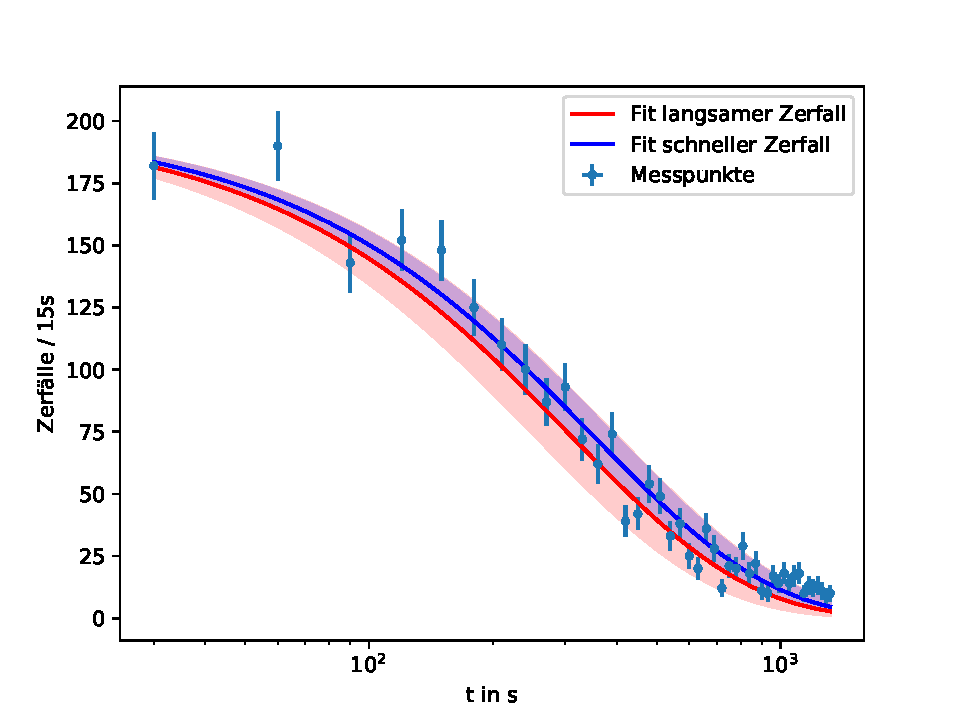
\includegraphics{Daten/Rhodium2.pdf}
	\caption{Messdaten und Fit für die Zerfallskurve von Rhodium.}
	\label{fig:zerfallskurve2}
\end{figure}